3D data acquired by sensors such as LiDARs and RGB-D (RGB point and depth value) cameras, complemented with 2D images, can make machines able to understand the surrounding environment; these data have rich geometric, shape and scale information and therefore have several areas of application, including autonomous driving, robotics, remote sensing and medical treatment~\cite{guo2020deep}.

Point cloud understanding includes many tasks, some of which are fundamental tasks in images, such as \textbf{classification}, that aims to assign to each object in the scene a category or class, \textbf{segmentation}, that is the task of labeling each individual point (it can be semantic or instance), and \textbf{object detection} recent research topic which objective is to locate all the objects in a given scene. Other tasks in point cloud are tracking (estimating the location of an instance in subsequent frames), flow estimation (estimating the flow among sequences of point clouds), matching and registration (finding the relationship between point clouds of the same scene collected in different ways), augmentation and completion (improving the quality of raw point clouds) and reconstruction.

In this survey we will describe some of the main existent approaches to point cloud classification.

\paragraph{Point Cloud}

A point cloud is a set of data points in space that may represent a 3D shape or object; each point is identified by a set of Cartesian coordinates $(x,y,z)$. 3D scanners or photogrammetry software produces sets of data by measuring many points on the surfaces of objects in their surrounding environment.

3D data can have different formats: depth images, point clouds, meshes and volumetric grids; point clouds representation is a very used format because it preserves the geometric information without discretization. In contrast to image data, point clouds don't directly contain spatial structure because they're composed by a set of 3D coordinates and they're not arranged in an array like images.

Deep learning techniques have recently been used to face many tasks in computer vision, especially image tasks; because of the difference between an image task and a 3D point cloud task, in order to apply deep learning to this type of data there are three main problems to be solved: find a dense representation from a sparse point cloud, build a network satisfying size-variance and permutation-invariance restrictions, process large volumes of data in lower time and computational resources \cite{lu2020deep}.

A general taxonomy of deep learning methods for 3D point clouds is illustrated in \ref{fig:taxonomy_point_clouds}: tasks can be divided in the three categories of classification, segmentation, and detection and tracking.

\begin{figure}[ht]
    \centering
    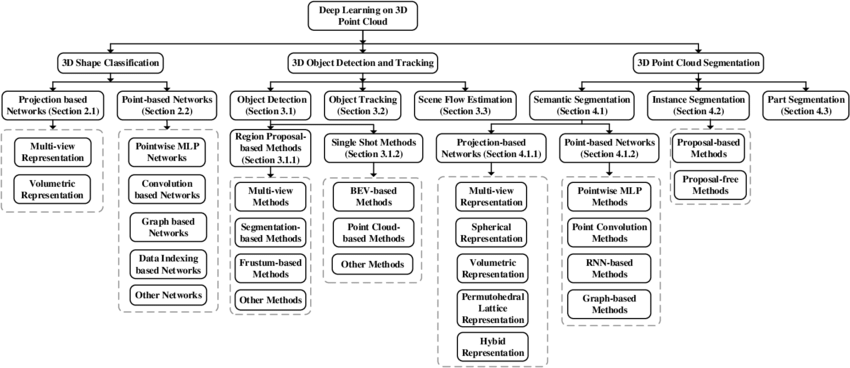
\includegraphics[width=0.8\textwidth]{images/taxonomy_point_clouds.png}
    \caption{A taxonomy of deep learning methods for 3D point clouds.}
    \label{fig:taxonomy_point_clouds}
\end{figure}

\paragraph{Classification task}

In this survey we will describe the task of classification on point clouds, since it's the first task to have been treated in the literature. Classification on point clouds is known as 3D shape classification and it's similar to image classification: methods usually learn the embedding of each point in the point cloud, then extract a global shape embedding for the whole cloud with an aggregation encoder; the global embedding is passed through fully connected layers to obtain the expected class. Classification models can be divided in projection-based methods and point-based methods, that will be illustrated in the next sections. Some important classification models in chronological order are shown in figure \ref{fig:chrono_deep} (\cite{guo2020deep}).

\begin{figure}[ht]
    \centering
    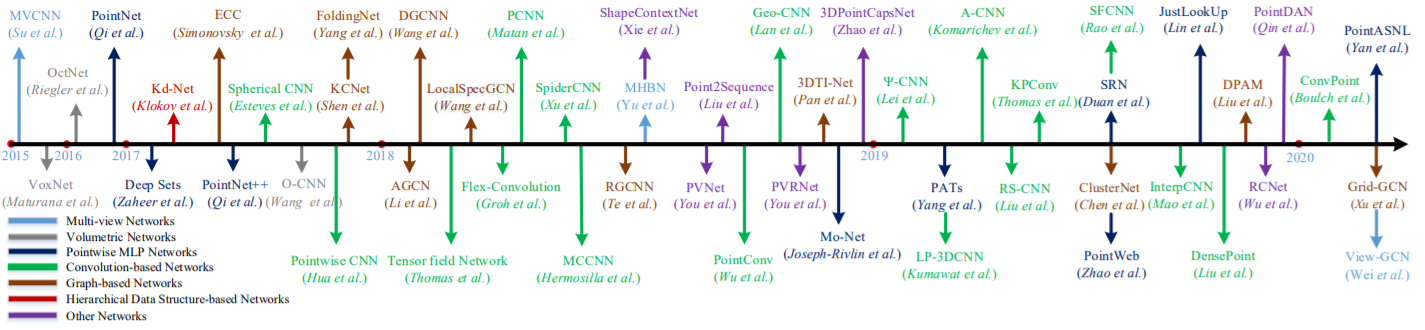
\includegraphics[width=0.9\textwidth]{images/chrono_deep.png}
    \caption{Relevant deep learning models for point cloud classification.}
    \label{fig:chrono_deep}
\end{figure}

\subsection{Datasets}
\label{subsec:datasets}

Well-designed datasets are needed to evaluate the performances of deep learning algorithm on 3D point clouds applications and help defining new tasks and research topics on the subject. 3D datasets are usually small because their capture requires much more effort than 2D images, and efficiently providing dense annotations in 3D is non-trivial~\cite{dai2017scannet}.

For the task of classification, datasets can be synthetic or real-world: the former are complete and don't have occlusions and background, the latter are occluded at different levels and some object are contamined with background noise. For the tasks of detection and tracking, datasets can be indoor scenes or outdoor urban scenes (used for autonomous driving).

\subsubsection{Synthetic datasets}

\paragraph{ModelNet40~\cite{ShapeNets}}
\label{ModNet40}
ModelNet is a large-scale object dataset of 3D computer graphics CAD models, constructed initially to train a 3D deep learning model called 3D ShapeNets. ModelNet is constructed from downloaded 3D CAD models labelled first with Amazon Mechanical Turk and then manually checked. It contains 151,128 3D CAD models belonging to 660 unique object categories. 

ModelNet project provides three benchmarks: ModelNet10, ModelNet40 and Aligned40 (where the numbers stand for the number of categories). Examples of classes and models of ModelNet40 are shown in figure \ref{fig:modelnet}.

This dataset, along with ShapeNet, is often used to evaluate the capacity of backbones before applying it to more complicated tasks. Since ModelNet40 is composed of CAD models and not point clouds, to use the points coordinates as input in the developped networks, the CAD models are sampled to reproduce point clouds. For example, to evaluate classification with PointNet, described later in section \ref{par:pointnet}, 1024 points are sampled uniformly from the mesh faces of the CAD models.

\begin{figure}[ht]
    \centering
    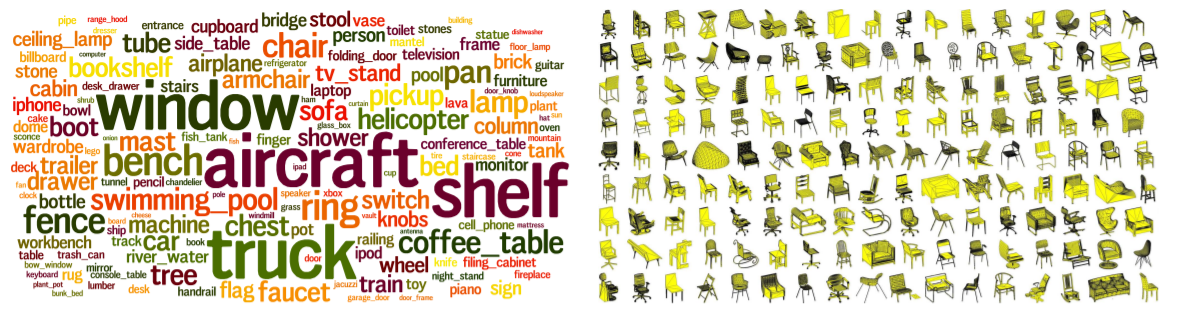
\includegraphics[width=0.9\textwidth]{images/modelnet.png}
    \caption{ModelNet40. Left: word cloud visualization of the ModelNet dataset. Right: examples of 3D chair models.}
    \label{fig:modelnet}
\end{figure}

\paragraph{ShapeNet~\cite{chang2015shapenet}}

ShapeNet is a repository of shapes represented by 3D CAD models for object of the everyday world, therefore it is a synthetic dataset of point clouds. It is richly-annotation and contains models spanning a multitude of semantic categories; there are 55 categories and they are organized in a hierarchical way according to WordNet synets ("synonym sets"). ShapeNet has a rich set of annotation for each shape and correspondences between them, the annotations are geometrice attributes such as orientation vectors, parts and keypoints, shape symmetries and scale of object in real world units.

The 3D model data comes from online repositories or existing research datasets, ShapeNet is intended to be an evolving dataset with regular updates. The objects are from the everyday world, so there are no CAD mechanical parts, molecular structures nor domain-specific objects. Figure \ref{fig:shapenet} shows some models from ShapeNet.

\begin{figure}[ht]
    \centering
    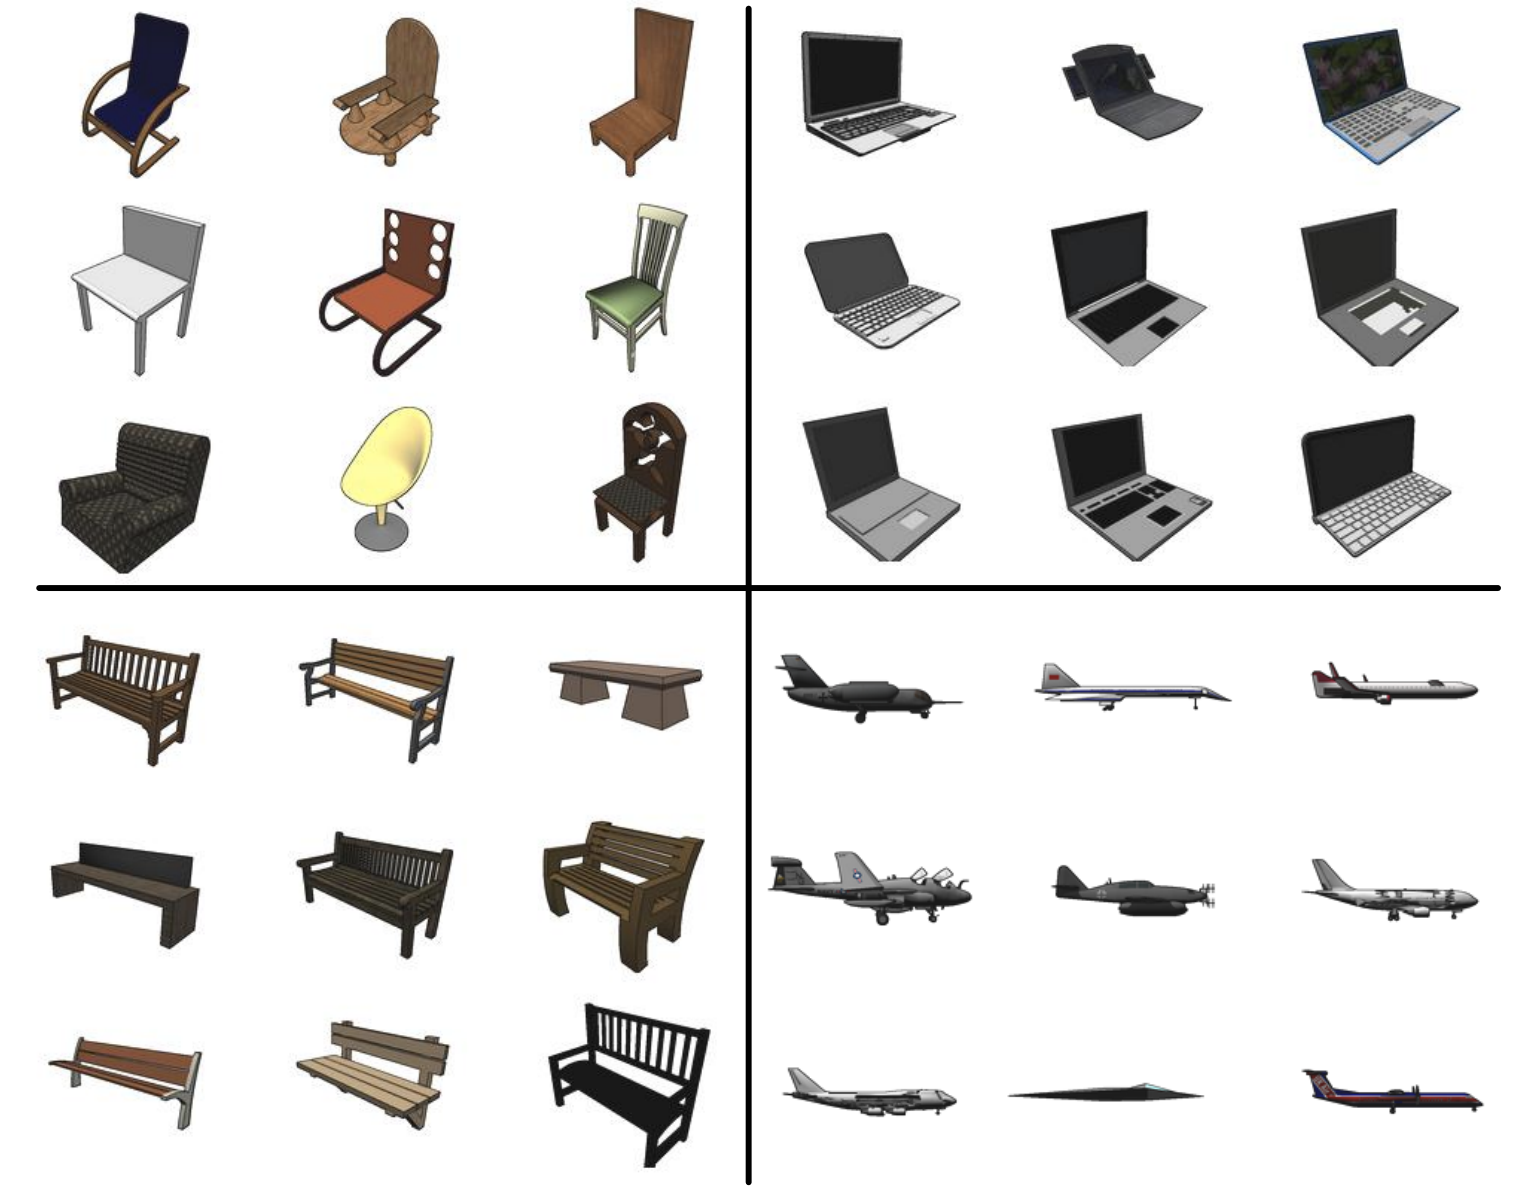
\includegraphics[width=0.5\textwidth]{images/shapenet.png}
    \caption{Some models of everyday world objects from the ShapeNet Dataset.}
    \label{fig:shapenet}
\end{figure}

The annotations in ShapeNet contain semantic information about the models, establish links between them and link to other modalities of data, such as images. There are different types of annotations: language-related annotations are synets from WorldNet taxonomy and they permit to name objects, for the aims of indexing, grouping and linking to related sources of data; geometric annotations represent objects from the structural point of view, they consist of rigid alignments, parts and keypoints, symmetries, and sizes; functional annotations describe the usage of represented objects, they are usually highly correlated with specific regions of an object, so they can include functional parts or affordances; physical annotations refer to fixed physical properties of objects such as dimension and densities, they can concert the surface material or the weight.

\subsubsection{Real-world datasets}

\paragraph{S3DIS~\cite{s3dis}}

S3DIS (Standford 3D Indoor Scene Dataset) is a large-scale dataset composed of colored 3D scans, that are points with 3D coordinated and RGB color values, of indoor areas of large building with various architectural styles. S3DIS contains 5 large-scale indoor scenes from three buildings. The point clouds are automatically generated without manual intervention.

The buildings are parsed into spaces that are semantically meaningful with a hierarchical parsing method. To parse point clouds into disjoint spaces the void-based approach was followed: the void spaces are detected using a density histogram and this forms a signature of the point cloud. Then, it was chosen a unique $xyz$ reference frame for the buildings, normalized in a cube. The disjoint spaces are then parsed into elements with labels.

\begin{figure}[ht]
    \centering
    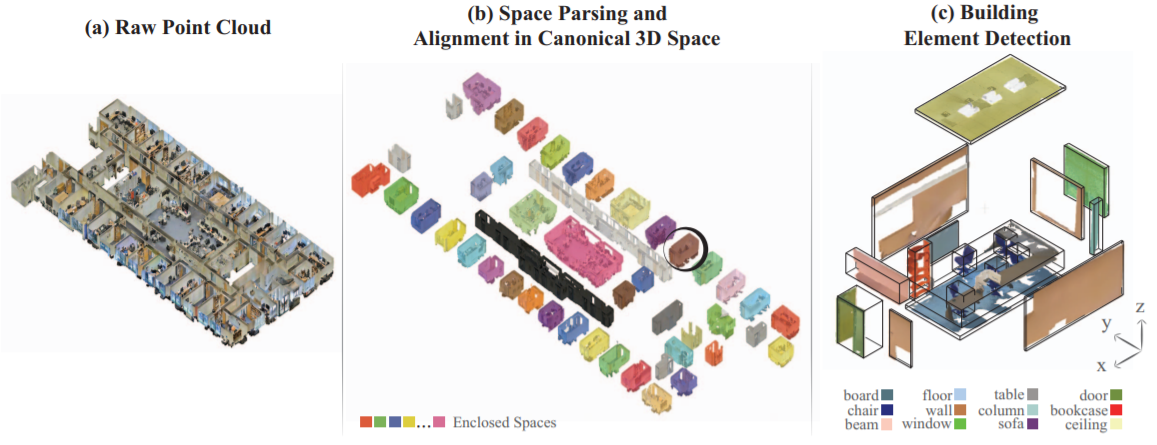
\includegraphics[width=0.8\textwidth]{images/s3dis.png}
    \caption{S3DIS: Semantic parsing of a large-scale point cloud.}
    \label{fig:s3dis}
\end{figure}

\paragraph{Semantic3D~\cite{hackel2017semantic3dnet}}

Semantic3D is the largest 3D point cloud dataset with terrestrial laser scans and semantic ground truth annotation, scenes are for example farms, town halls, sport fields, castles and market squares. It has over 4 billions points  collected from around 110000 $m^2$ area with a static LiDAR, and class labels for 8 classes (man made terrain, natural terrain, high vegetation, low vegetation, buildings, remaining hard scale, scanning artifacts, cars and trucks).

The class labels have been manually assigned to each point, this strategy permitted to not inherit errors from the segmentation approach. The manual labelling can be done in 3D, selecting few points and fitting a simple model to label the object, or in 2D, rotating the point cloud to fix a view and draw closed polygons to detect objects.

\paragraph{ScanNet~\cite{dai2017scannet}}

It is a dataset of richly-annotated RGB-D scans of real-world environments containing 2.5 millions RGB-D images in 1513 scans acquired in 707 distinct spaces; this dataset is annotated with estimated calibration parameters, camera poses, 3D surface reconstructions, textured meshes, dense object-level semantic segmentations, and aligned CAD models. ScanNet contains spaces such as offices, apartments, and bathrooms, ranging from small to large spaces.

Data are collected as videos through handheld devices such as iPhone or iPad with an attached RGB-D sensor. The semantic annotation is done with Amazon Mechanical Turk for instance-level object category labeling and 3D CAD model alignment. The framework used to acquire data runs in an unsupervised way so it continues to grow.

\paragraph{KITTI~\cite{kitti}}

KITTI is among the most famous benchmarks with 3D data. Data are captured from a VW station wagon, an autonomous driving platform with two high-resolution color and grey cameras, a Velodyne laser scanner and a GPS localization system, for use in mobile robotics and autonomous driving research, data are used for 3D object detection, tracking and scene flow estimation. Scenarios include real-world traffic on freeways in rural areas or inner-city scenes with many static and dynamic objects.

The dataset includes camera images, laser scans, high-precision GPS measurements and IMU accelerations (i.e. a specific type of sensor that measures angular rate, force and sometimes magnetic field) from a combined GPS/IMU system. The raw data are divided into the categories 'Road', 'City', 'Residential', 'Campus' and 'Person'; for each sequence data include raw data, object annotations in form of 3D bounding box tracklets and a calibration file. For each dynamic object within the reference camera's field of view, the 3D bounding boxes classify objects in the classes 'Car', 'Van', 'Truck', 'Pedestrian', 'Person', 'Cyclist', 'Tram' and 'Misc'; each object has a class and its 3D size. For each frame it's available the object's translation and rotation in 3D in the Velodyne coordinates, along with the level of occlusion and truncation.

\paragraph{nuScenes~\cite{caesar2020nuscenes}}

nuScense (nuTonomy scenes) carries the full autonomous vehicle sensor suite: 6 cameras, 5 radars and 1 LiDAR, all with full 360 degree field of view. The dataset includes 1000 scenes of 20 seconds, each fully annotated with 3D bounding boxes from 23 classes and 8 attributes, The scenes include high traffic density such as intersections and construction sites, rare classes such as ambulances and animals, potentially dangerous traffic situations, such as jaywalkers or incorrect behaviors, maneuvers such as lane change, turning and stopping, and difficult situations for computer vision. The scenes are annotated by expert annotators with textual descriptions. Every object in a keyframe sampled from the scenes is labelled by experts with one of the 23 classes, semantic categories, and attributes (visibility, acitivity and pose), and a cuboid with $xyz$ coordinates, width, length, height and yaw angle.

\paragraph{WaymoOpen~\cite{sun2020scalability}}

This dataset consists of 1150 scenes of 20 seconds each, consisting of 5 LiDAR sensors and 5 pinhole camera data captured in urban and suburban geographies; data are annotated with 2D and 3D bounding boxes. For every label in LiDAR and camera data the dimensions of bounding boxes are defined.

\begin{figure}[ht]
    \centering
    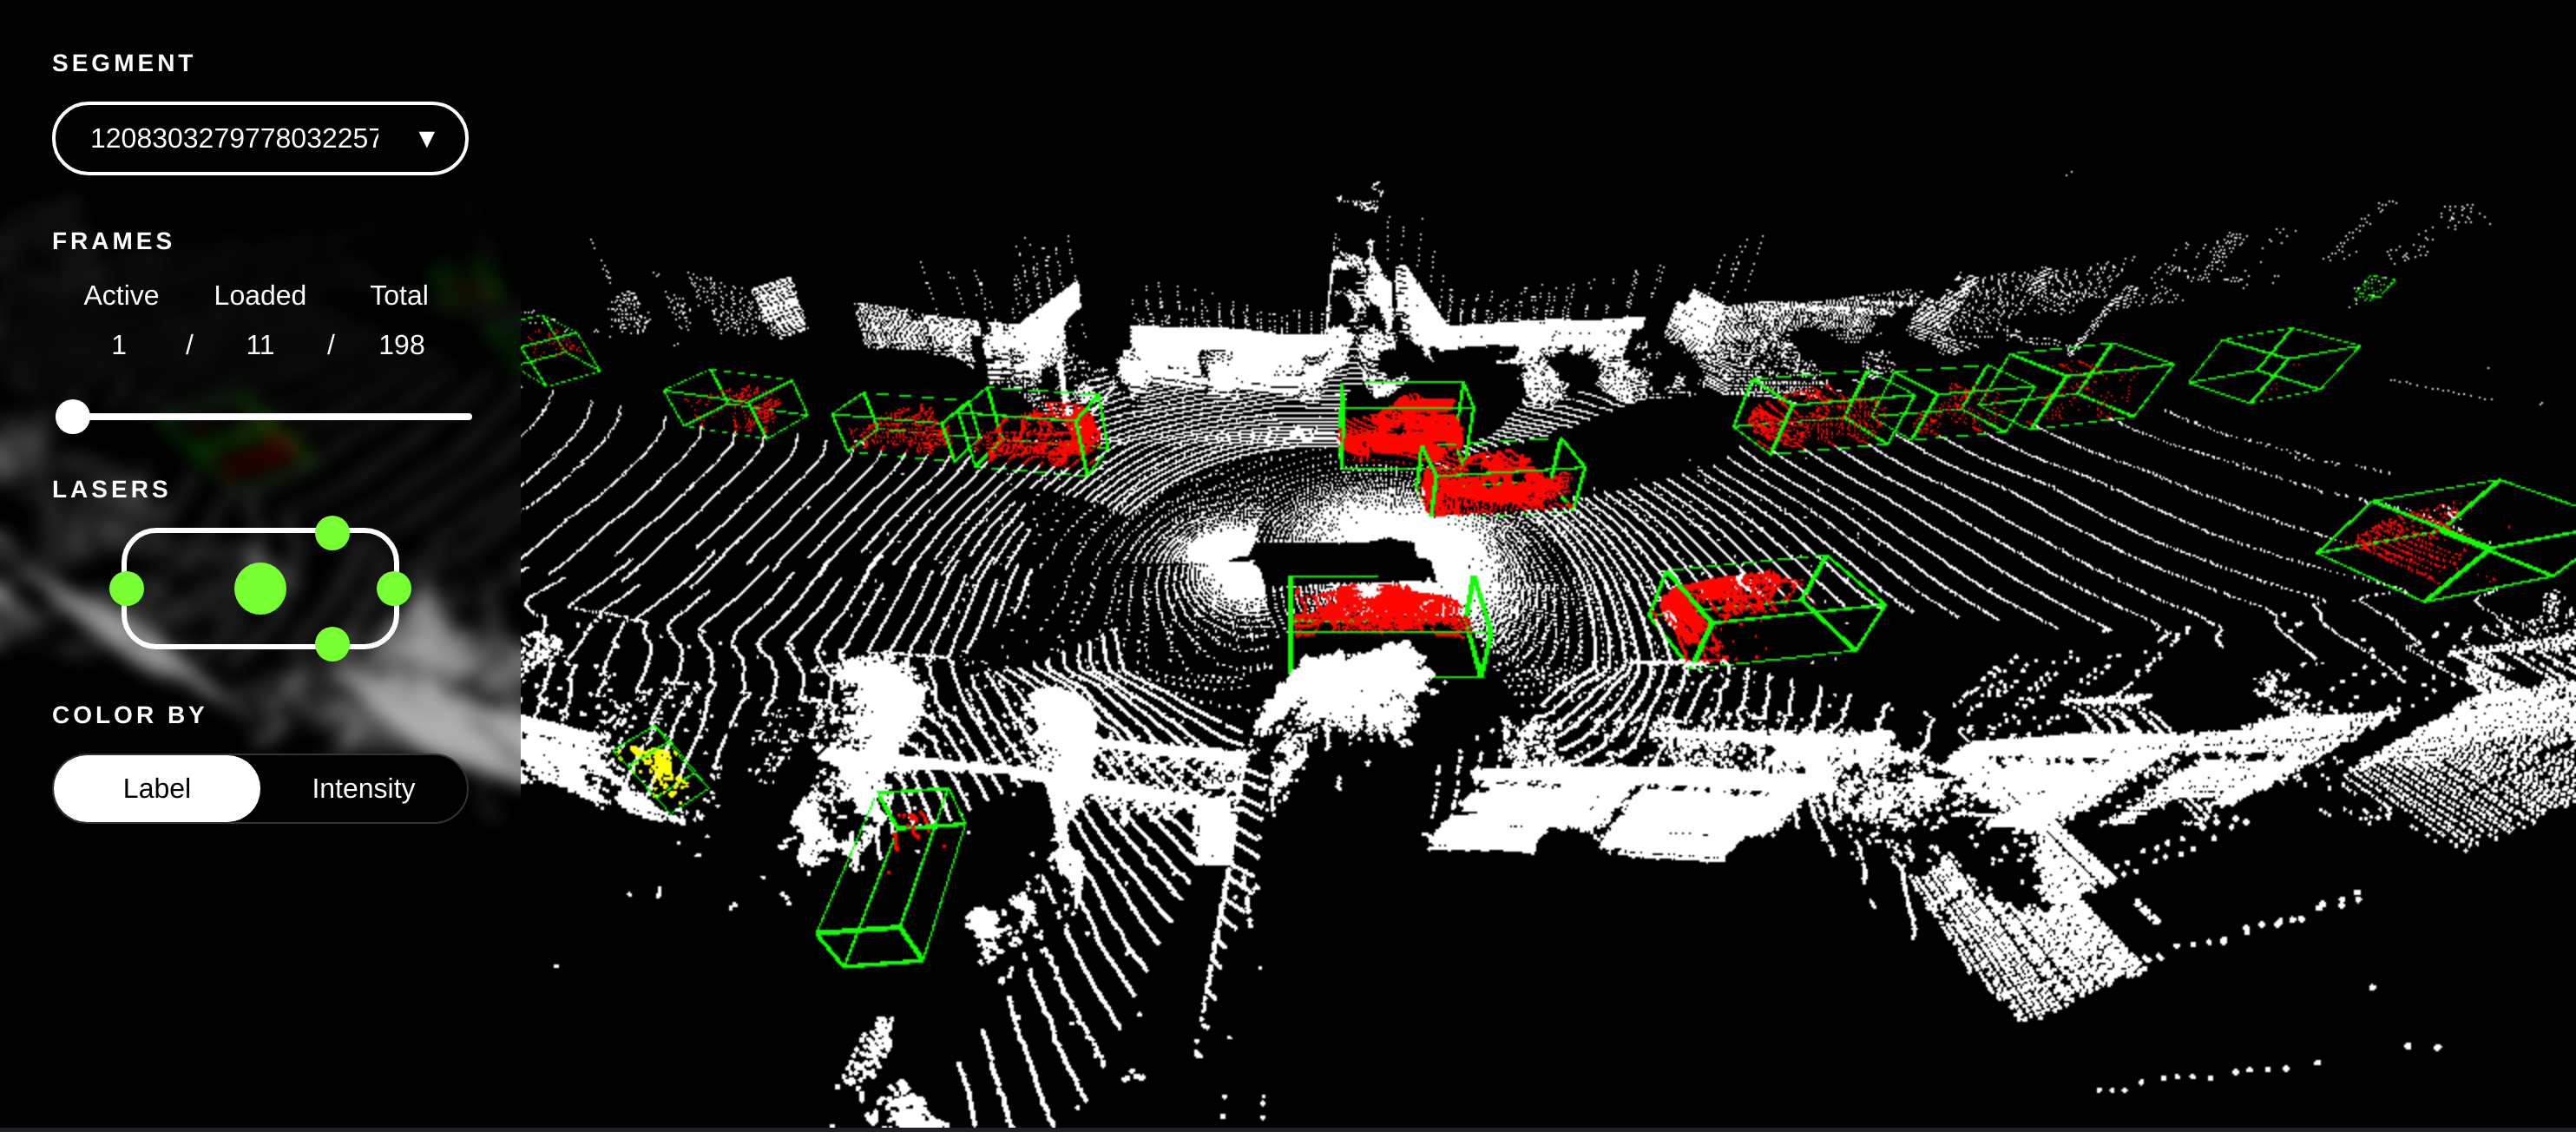
\includegraphics[width=0.8\textwidth]{images/waymo.png}
    \caption{LiDAR label example in Waymo dataset.}
    \label{fig:waymo}
\end{figure}

Vehicles, pedestrians, signs and cyclist in LiDAR data are exhaustively annotated: every object is labeld with $cx$, $cy$, $cz$, the center coordinated, $l$, $w$, $h$, the length, width and height, $\alpha$, the heading angle of the bounding box. Vehicles, pedestrians and cyclist are also annotated in camera data, with a bounding box defined by $cx$, $cy$, $l$, and $w$.

\subsection{Metrics}
\label{subsec:metrics}

Metrics are needed in order to compare performances of different algorithms; different evaluation metrics have been proposed for every task in point cloud understanding, so it is important to choose the appropriate ones (\cite{lu2020deep}, \cite{guo2020deep}).

For the task of \textbf{3D shape classification} the most commonly used metrics are the \textit{Overall Accuracy (O.A.)} and the \textit{Mean Class Accuracy (mACC)}. The O.A. is the fine as the accuracy on the entire dataset and indicated how many predictions are correct over all predictions:

\[O.A. = \frac{TP+TN}{|dataset|}=\frac{TP+TN}{TP+TN+FP+FN}\]

mACC is the mean of accuracy of the accuracy of every class:

\[mACC = \frac{1}{C} \sum\limits_{c=1}^C Accuracy_c\]

where $C$ is the number of classes in the dataset.

% The task of \textbf{3D point cloud segmentation} shares with the previous one two metrics, that are O.A. and mAcc, but it's common to use \textit{Mean Intersection Over Union (mIoU)}, too. Intersection Over Union, or IoU, used often on bounding boxes, is defined as the ratio between the area of overlap between two bboxes (intersection) and the area of union between the two bboxes. The mIoU is defined as the mean of IoU on all classes.

% Other used metrics, common also in other point cloud understanding tasks, are \textit{Precision} and \textit{Success} and their average counterpart. They are defined as:

% \[\begin{array}{c}
%      Precision = \frac{TP}{TP+FP}  \\
%      \\
%      Recall = \frac{TP}{TP+FN}
% \end{array}\]

% In other tasks such as 3D single and multi-object tracking two used metrics are \textit{AMOTA (Average Multi-Object Tracking Accuracy)}, \textit{AMOTP (Average Multi-Object Tracking Precision)}. In \textbf{Scene estimation} and \textbf{3D match and registration} commonly used metrics are \textit{End Point Error (EPE)} and \textit{ROC Curves}.

% In addition to these techniques, it is always suggested to visualize result as it is always an effective supplement of numbers.
  